\chapter{Управление бесколлекторным двигателем}
\label{cha:chap1}

\section{Устройство двигателя и принцип работы}
\label{sec:bldc_theory}

В основе коллекторных двигателей постоянного тока лежит механический механизм коммутации обмоток с использованием щёток, изменяющим направление тока в обмотках якоря для формирования постоянного момента. Из-за этого возникают электромагнитные и акустические шумы, появляется потребность в довольно частом обслуживание щеточно-коллекторного узла из-за износа, возникающего в следствии трения механических частей и искрения в процессе коммутации. \cite{book.kim_motors}

Чтобы преодолеть эту проблему, были разработаны бесколлекторные двигатели (БДПТ). По своей структуре они являются синхронными двигателем с сосредоточенным распределением и магнитоэлектрическим возбуждением обмоток статора, но которые питаются от постоянного тока. В данном типе двигателей коммутация обмоток происходит не механическим способом (как в коллекторных двигателях), а электрическим. Для электрической коммутации зачастую ипользуются датчики положения ротора и специализированные управляющие схемы на основе управляемых ключей (транзисторов). \cite{book.itmo_motors,book.kim_motors}

\begin{figure}[!h]
\centering
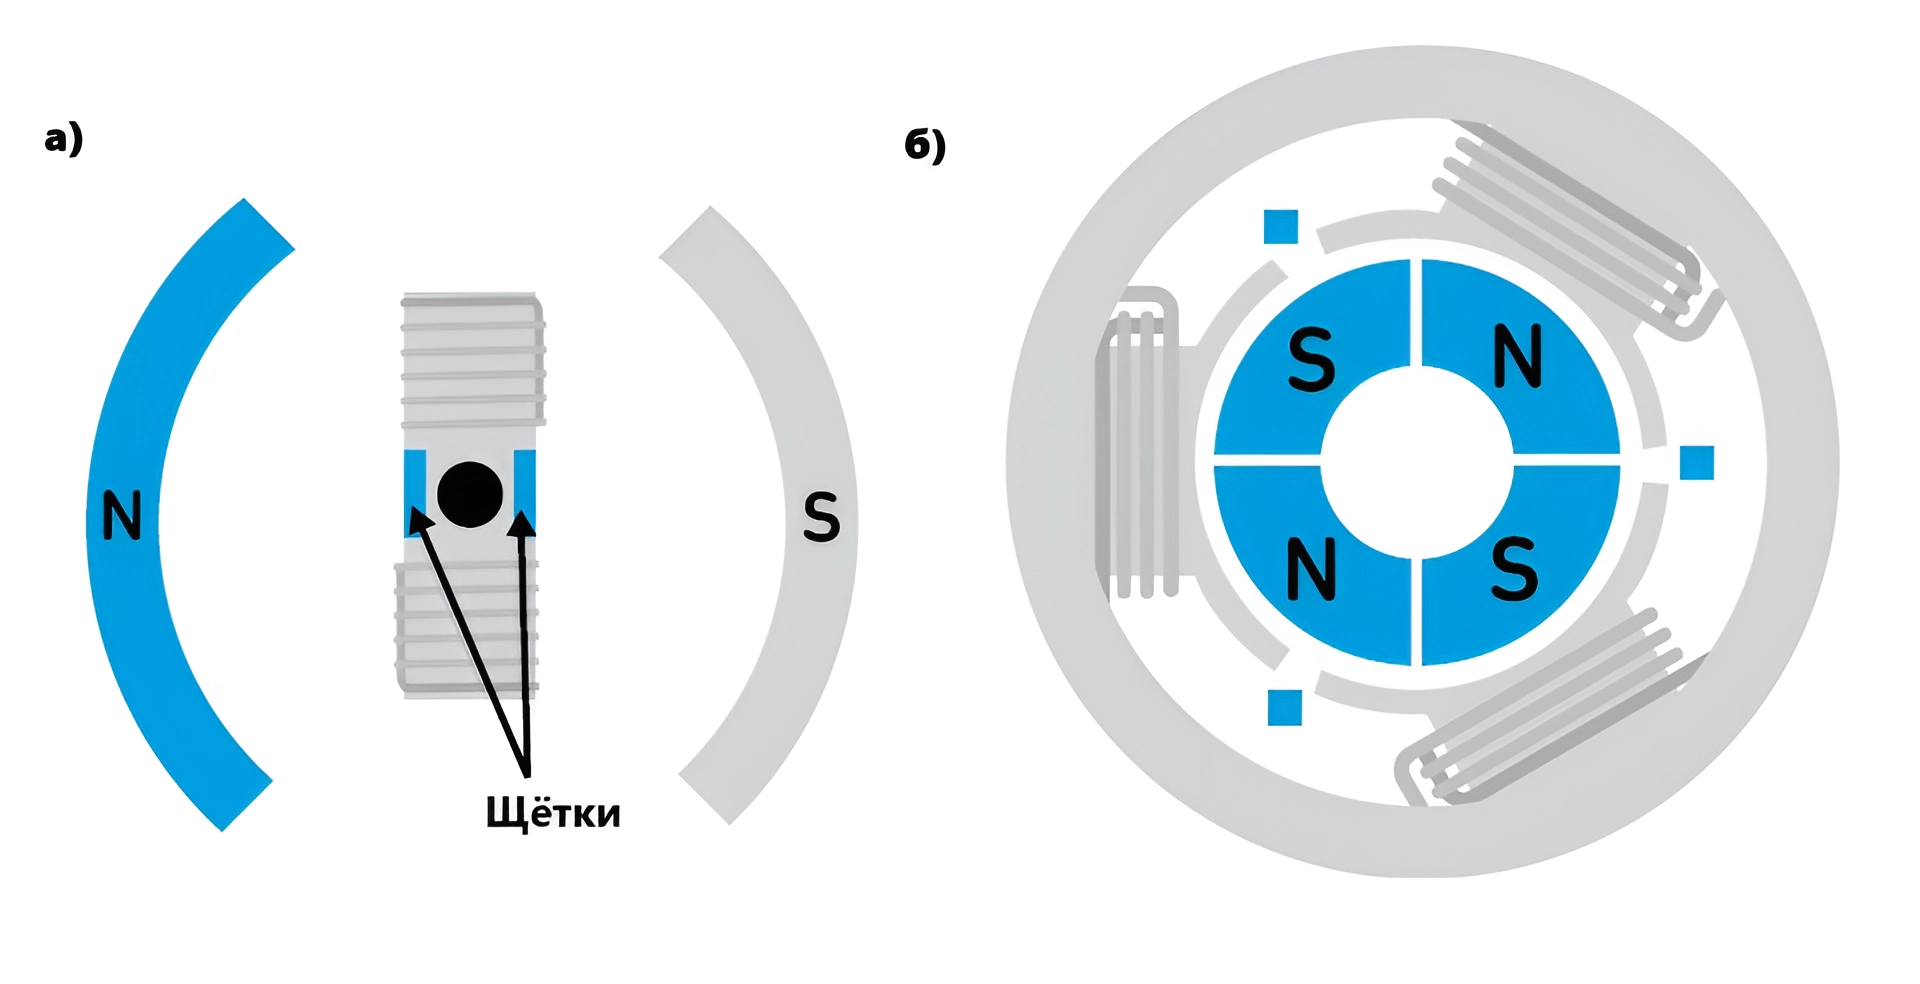
\includegraphics[width=0.7\textwidth]{inc/img/dc_and_bldc.png}
\caption{Структура двигателей постоянного тока: а - коллекторный дпт, б - бесколлекторный дпт \cite{book.bldc_dummy}}
\end{figure}

Благодаря своей структуре бесколлекторные двигатели постоянного тока обладают большей эффективностью из-за меньших затрат на коммутацию, большей надёжностью из-за отсутствия щеточно-коллекторного узла, меньшими габаритами при сравнимой мощности (большей плотностью мощности) и меньшей стоимостью из-за более простой конструкциии в сравнении с традиционными двигателями постоянного тока.

Стоит также отметить отличия БДПТ от синхронных машин с постоянными магнитами (также называются вентильными двигателями или синхронными машинами с постоянными магнитами), которые имеют распределённую обмотку статора и питаются от переменного тока, из-за чего имеют синусоидальный характер противо-ЭДС в обмотках. Тогда как в БДПТ она имеет трапецеидальный характер (Рисунок \ref{img:eds}). Ввиду этих особенностей к этим двигателям применяются разные алгоритмы управления и разные драйверы. Для вентильных двигателей алгоритмы управления зачастую имеют более сложный характер.

\begin{figure}[!h]
\centering
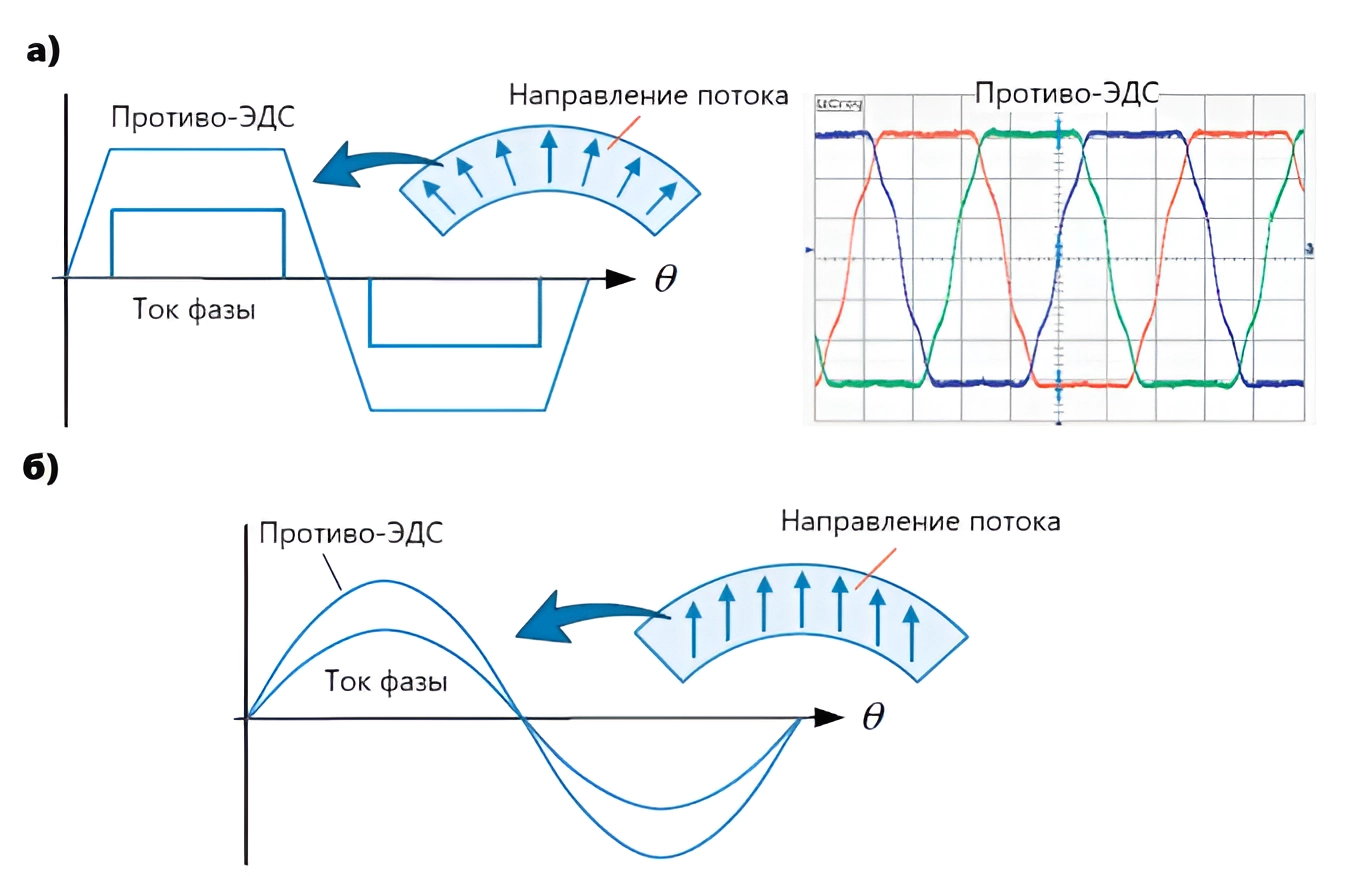
\includegraphics[width=0.7\textwidth]{inc/img/bldc_and_pmsm.png}
\caption{Вид противо-ЭДС: а - бесколлекторный дпт, б - вентильный двигатель \cite{book.kim_motors}}
\label{img:eds}
\end{figure}

\section{Управление на основе датчиков Холла}
\label{sec:hall}
БДПТ можно представить в виде трёх соединенных между собой обмоток. Одновременно можно пропускать ток через 2 из 3 обмоток, что позволяет создать 6 направлений вектора магнитного поля статора, представленных на Рисунке \ref{img:mag_field}.

\begin{figure}[!h]
\centering
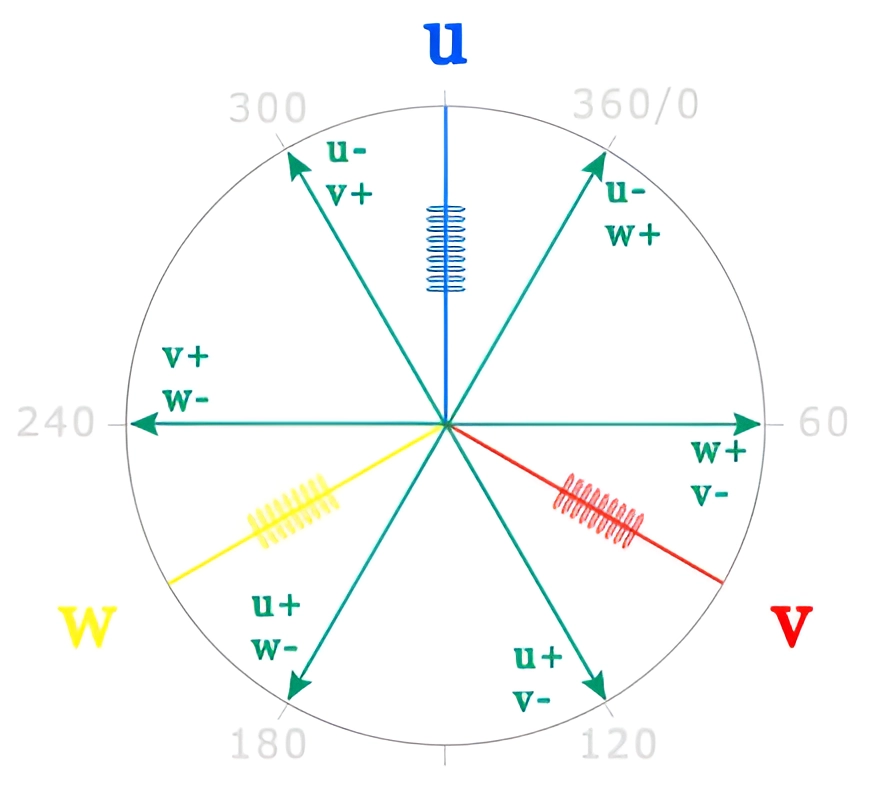
\includegraphics[width=0.7\textwidth]{inc/img/bldc_vec.png}
\caption{Возможные направления векторов магнитного поля, создаваемого статором bldc двигателя (U, W, V --- выходы обмоток двигателя) \cite{habr:bldc_control}}
\label{img:mag_field}
\end{figure}

Таким образом, для управления необходимо вовремя коммутировать фазы обмоток, создавая круговое магнитное поле. Из этого можно получить закон коммутации из 6 шагов (число которых соотвествует числу возможных комбинаций протекания тока через обмотки). Возможная последовательность коммутации обмоток приведена в Таблице \ref{table:commutation}.

\clearpage
\begin{center}
\captionof{table}{Возможная таблица коммутации обмоток (U, W, V --- выходы обмоток двигателя)\label{table:commutation}}
\begin{tabular}{|c|c|c|}
 \hline
 DC + & DC - & Не подключена \\
 \hline
 W & U & V \\ 
 \hline
 W & V & U \\
 \hline
 U & V & W \\
 \hline
 U & W & V \\
 \hline
 V & W & U \\
 \hline
 V & U & W \\
 \hline
\end{tabular}
\end{center}

Но как можно определить момент, в который необходимо изменить направление протекания тока в обмотках (перейти к следующему шагу цикла)? Самое простое в плане реализации системы управления является установка специальных датчиков, работающих на эффекте Холла. Они обычно располагаются под $120$ электрических градусов друг от друга, чтобы за один цикл коммутации получить все возможные комбинации состояний датчиков (кроме состояний, когда все сработали или ни один не сработал, что невозможно в работающем двигателе из-за их расположения). Стоит отметить, что $360$ электрических градусов соответствуют одному периоду магнитного поля или одному выполнению цикла коммутации.

Для определения механических градусов (то есть расположения на самом статоре) необходимо знать число пар полюсов двигателя ($N$) и воспользоваться формулой: $\dfrac{360}{3N}$. Например, в однополюсном двигателе датчики располагаются под углом в $120^{\circ}$, в двухполюсном --- $60^{\circ}$ и т. д. Из этого следует, что для одного механического оборота двигателя необходимо выполнить количество циклов коммутации, равное числу пар полюсов двигателя.

\begin{figure}[!h]
\centering
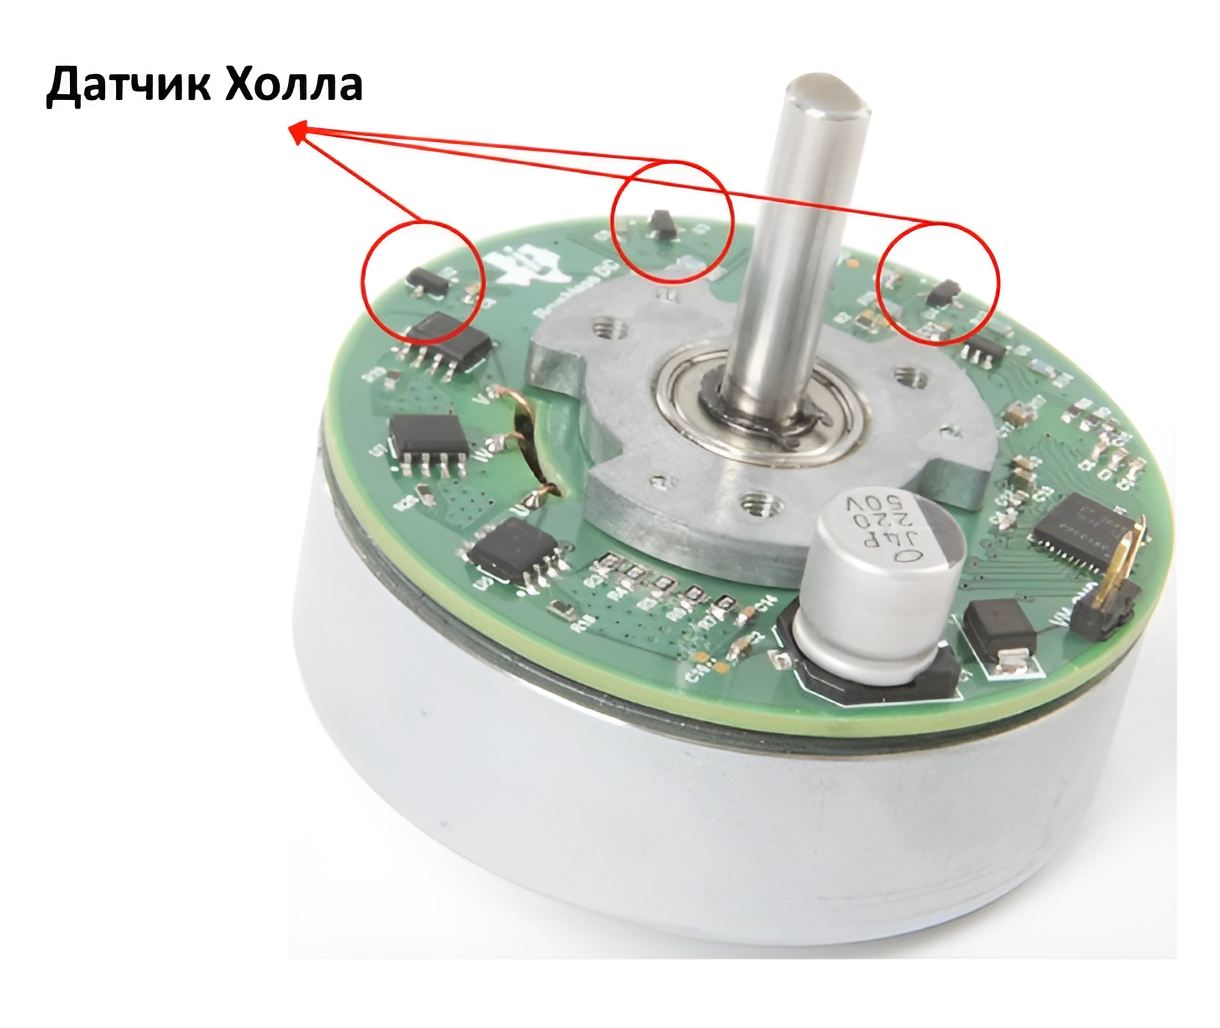
\includegraphics[width=0.7\textwidth]{inc/img/hall.png}
\caption{Возможное расположение датчиков Холла}
\end{figure}

\section{Особенности бездатчикового управления}
\label{sec:sensorless_ways}

Можно ли определить позицию ротора без использования специальных датчиков, которые удорожают конструкцию и образуют ещё один узел, который надо обслуживать, и который может выйти из строя? Для этой цели используется бездатчиковое управление, которое сейчас набирает всё большую популярность в связи с развитием вычислительной техники.

Самым популярным способом для организации такого управления является использование обратной связи по противо-ЭДС. Т. к. одновременно ток протекает только через две обмотки, то на третьей обмотке индуцируется напряжение, возникающее при взаимодействии с магнитным полем, по которому можно определить положение ротора. После чего можно использовать таблицу коммутации, рассмотренную в \ref{sec:hall}.

Как было отмечено в \ref{sec:bldc_theory}, противо-ЭДС в бесколлекторным двигателях имеет трапецеидальную форму, но это не сильно важно, ведь зачастую нужно отслеживать только точки пересечения характеристикой нуля. Моменты переключения фаз показаны на Рисунке \ref{pic:sensorless_commut}.

\begin{figure}[!h]
\centering
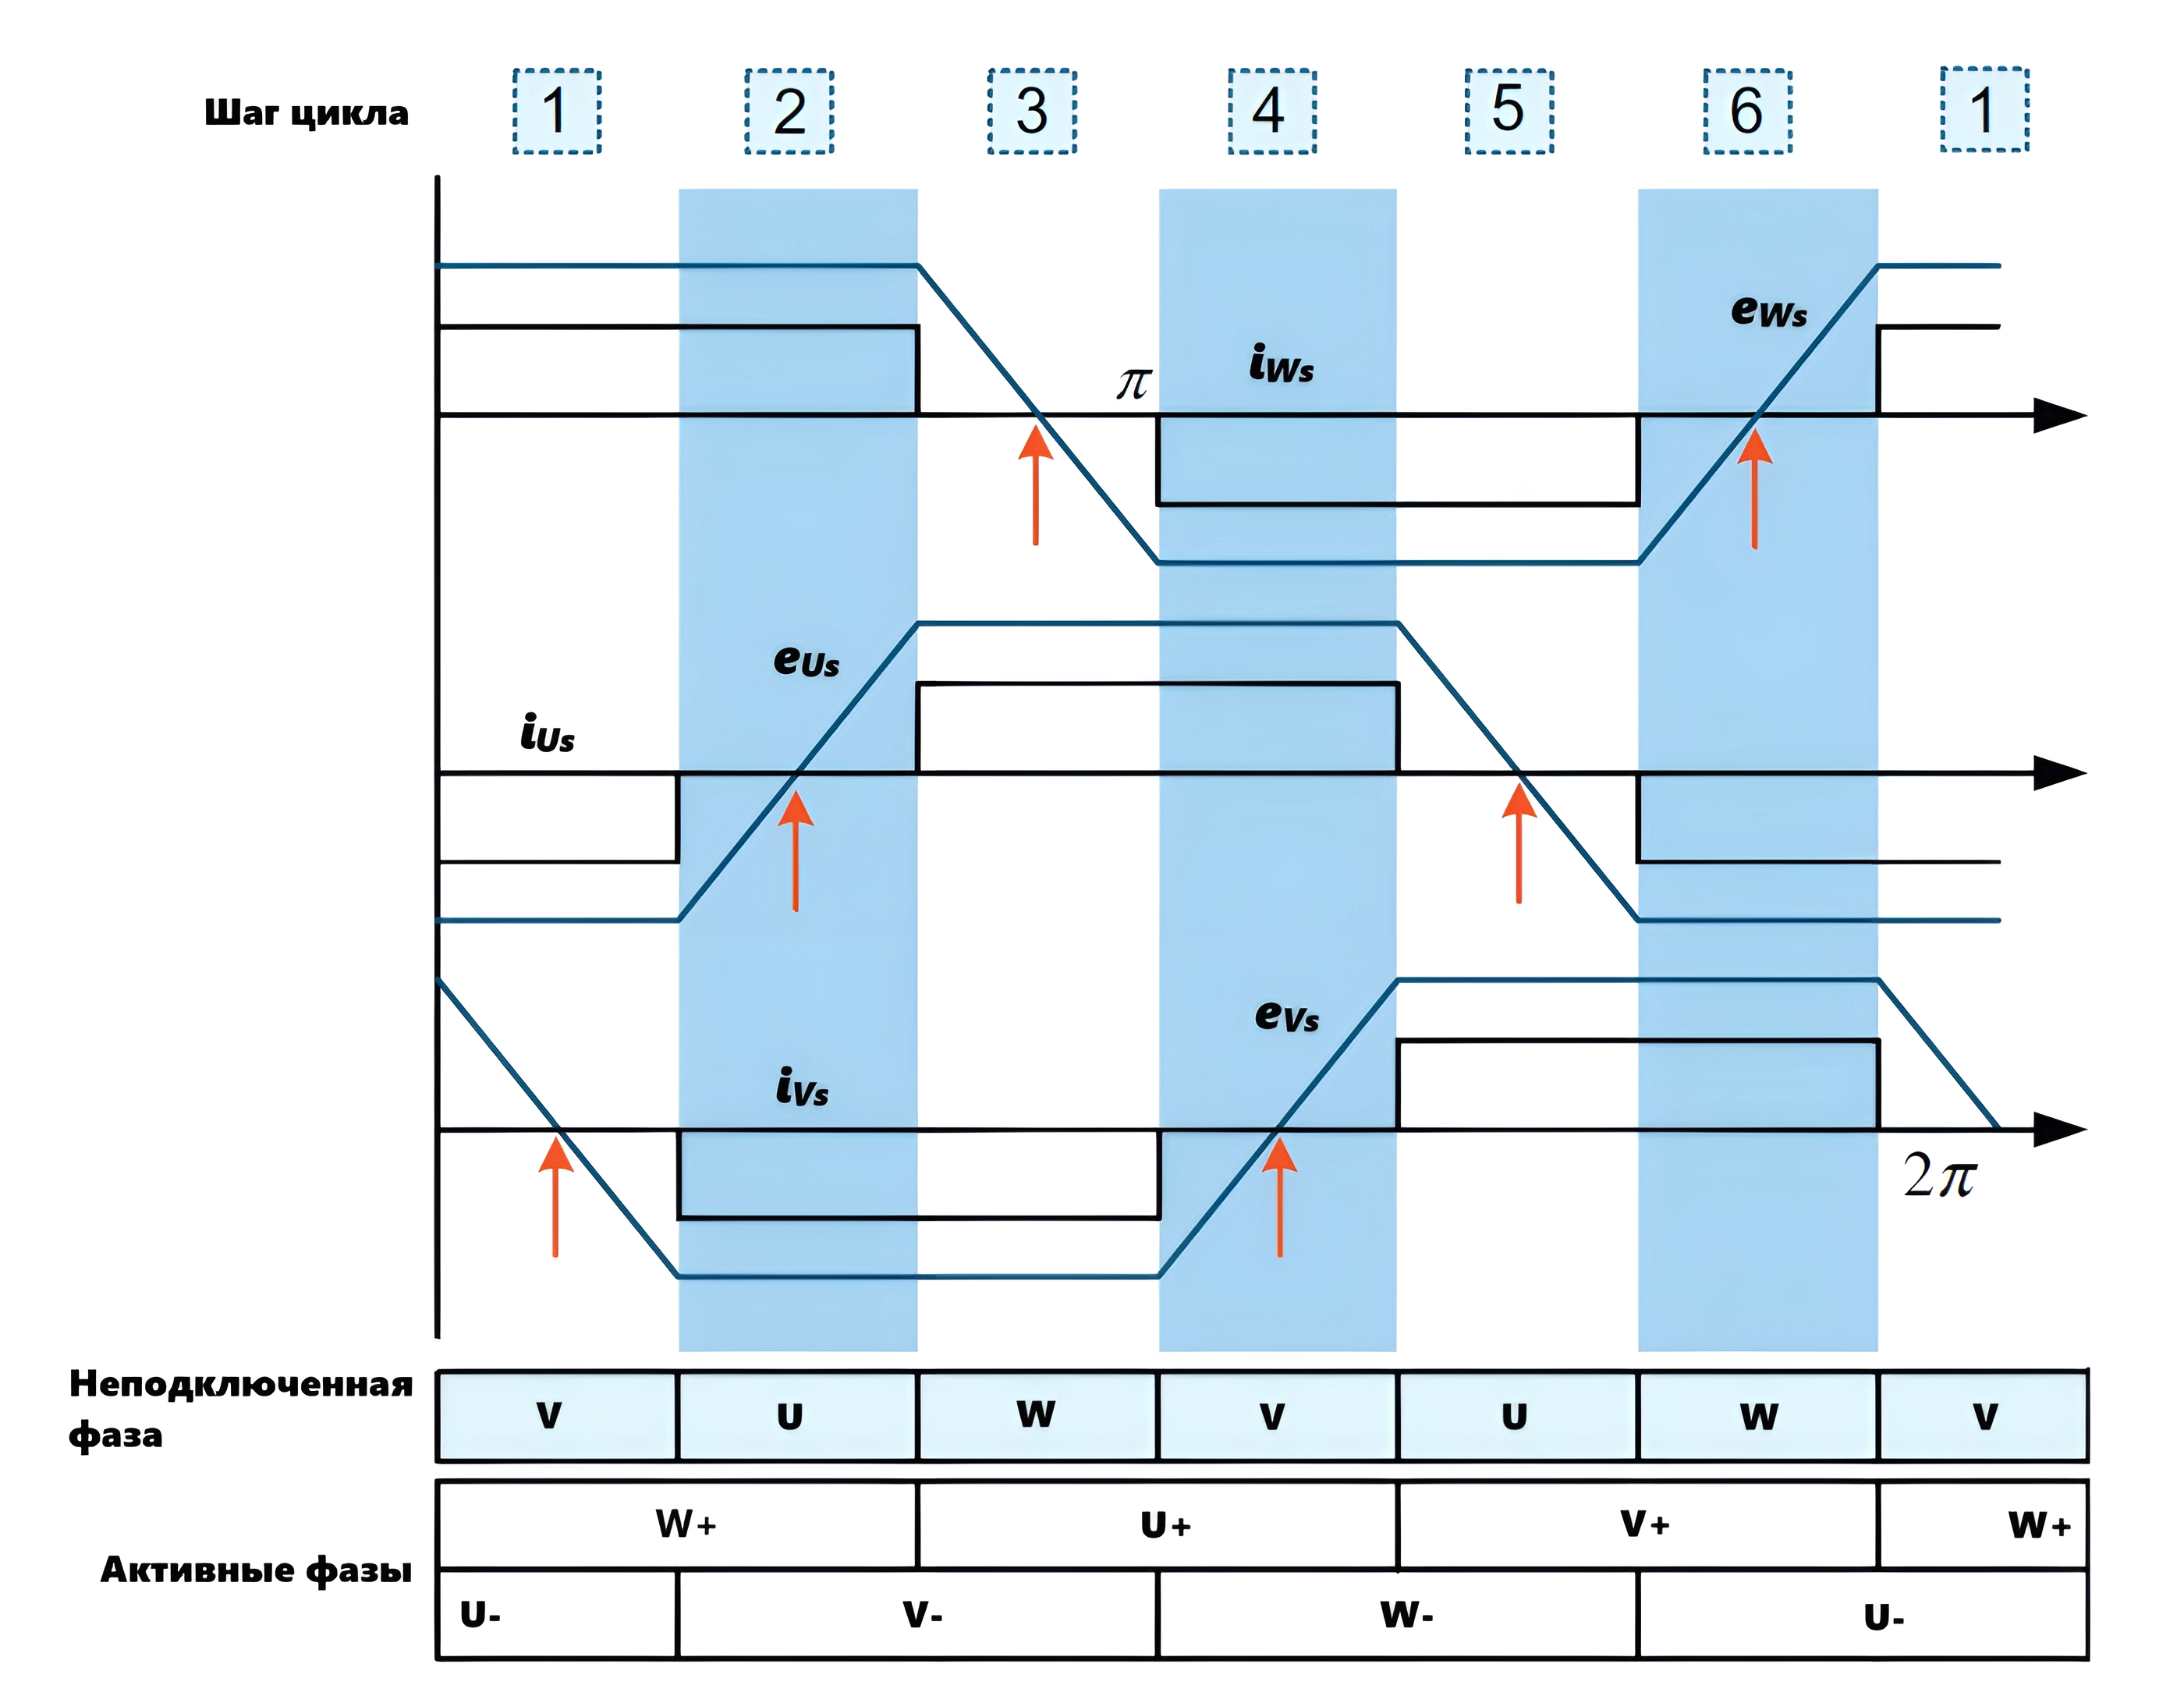
\includegraphics[width=\textwidth]{inc/img/sensorless_commut.png}
\caption{Переключение фаз в точках пересечения нуля противо-ЭДС ($e$ --- противо-ЭДС фазы, $i$ --- ток фазы)}
\label{pic:sensorless_commut}
\end{figure}
\clearpage

Но не всё так гладко: на практике особенно на низких скоростях бывает сложно засечь точку пересечения нуля, т. к. уменьшается амплитуда противо-ЭДС, что делает данный метод неработоспособным при необходимости управления на околонулевых скоростях, тем более в условиях шумов. В этом случае обычно цикл коммутации выполняют просто с каким-то интервалом до тех пор, пока не выйдут на скорость, достаточную для точного определения положения по противо-ЭДС (выполняется <<слепой>> старт).

Другие методы для определения позиции ротора без использования датчиков \cite{art:bldc_sensorless}:
\begin{enumerate}
	\item расчёт потокосцепления из уравнения двигателя по известным величинам тока, напряжения и сопротивления $\left(V=Ri+\dfrac{d}{dt}\Psi\right)$ и соотнесения его величины с позицией ротора;
	\item построение наблюдателя противо-ЭДС и последующее вычисление положения и скорости ротора (например, использование наблюдателя Люенбергера или наблюдателя на основе скользящих режимов).
\end{enumerate}



